% % % % % % % % % % % % % % % % % %
%DGL 1. Ordnung - Orthogonaltrajektorien
% % % % % % % % % % % % % % % % % %	
\begin{tabularx}{\textwidth}{|p{100pt}|X|}
	\hline
	\rowcolor{Gray}
	\multicolumn{2}{|c|}{\textbf{DGL 1. Ordnung}}\\
	\hline
		Orthagonaltrajektorien \newline
		
		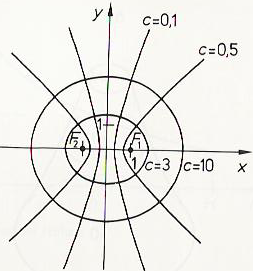
\includegraphics[width = 90pt]{bilder/orthoTrajekt_klein.png}	
		
		&
		Orthogonaltrajektorien sind die Normalen der DGL. Sie stehen senkrecht auf den Kurven die durch die DGL entstehen. \newline
		Die orthogonalen Trajektorien schneiden alle Kurven der gegebenen Kurvenschar
		$y=f(x,c)$ im rechten Winkel. \newline
					\textbf{Vorgehen:}
					\begin{compactenum}
						\item $y$ nach $c$ umstellen/ auflösen
						\item $y$ ableiten $\Rightarrow y'$
						\item in $y'$ Gleichung (entweder oder)
						$\begin{cases}
							c \text{ substitutieren/ ersetzen} \Rightarrow \text{DGL: F(x,y,y')}\\
							y \text{ Gleichung in } y' \text{ Gleichung einsetzen}
						\end{cases}$
						\item $y'$ durch $-\frac{1}{'y}$ ersetzen.
						\item DGL auflösen (sofern nötig...)
					\end{compactenum}
				\begin{minipage}{0.2\textwidth}
					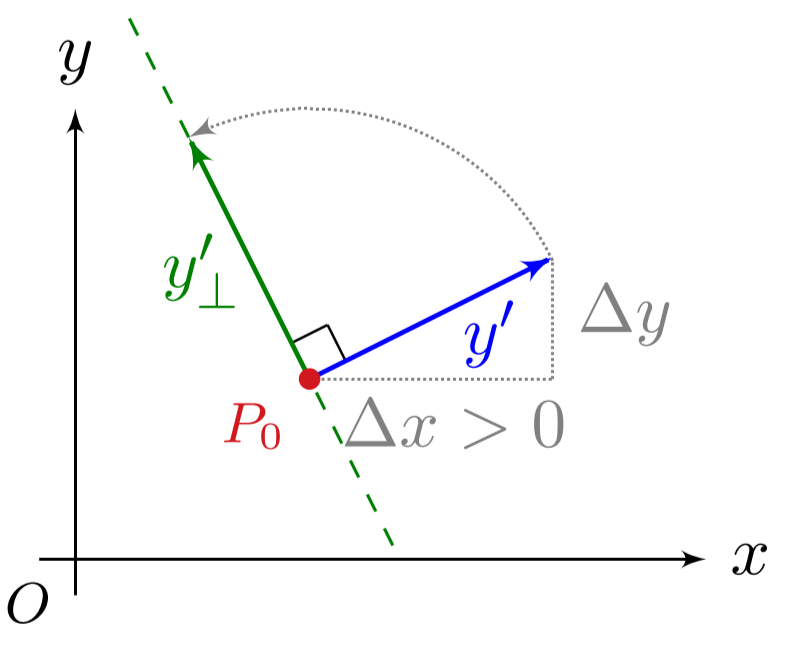
\includegraphics[width = \textwidth]{bilder/orthoTrajekt_Formel}
				\end{minipage} 
				\begin{minipage}{0.3\textwidth}
					\begin{tabular}{c|c}
						Kartesische Koordinaten: & Polarkoordinaten \\
						$y^{\prime}=f(x, y) \quad \Rightarrow \quad y_{\perp}^{\prime}=-\frac{1}{f(x, y)}$ &
						$r^{\prime}=f(r, \varphi) \quad \Rightarrow \quad r_{\perp}^{\prime}=-\frac{r^{2}}{f(r, \varphi)}$
					\end{tabular}
				\end{minipage}
				
				\\
	\hline
\end{tabularx}
		%		\end{minipage}%
%		\begin{minipage}{.8\textwidth}
%			Die orthogonalen Trajektorien schneiden alle Kurven der gegebenen Kurvenschar
%			$y=f(x,c)$ im rechten Winkel.\\

%		\end{minipage}



\end{center}
\end{table}	
